\documentclass[a4paper]{article}
\usepackage[utf8]{inputenc}
\usepackage[spanish, es-tabla, es-noshorthands]{babel}
\usepackage[table,xcdraw]{xcolor}
\usepackage[a4paper, footnotesep = 1cm, width=20cm, top=2.5cm, height=25cm, textwidth=18cm, textheight=25cm]{geometry}
%\geometry{showframe}

\usepackage{tikz}
\usepackage{amsmath}
\usepackage{amsfonts}
\usepackage{amssymb}
\usepackage{float}
\usepackage{graphicx}
\usepackage{caption}
\usepackage{subcaption}
\usepackage{multicol}
\usepackage{multirow}
\setlength{\doublerulesep}{\arrayrulewidth}
\usepackage{booktabs}

\usepackage{hyperref}
\hypersetup{
    colorlinks=true,
    linkcolor=blue,
    filecolor=magenta,      
    urlcolor=blue,
    citecolor=blue,    
}

\newcommand{\quotes}[1]{``#1''}
\usepackage{array}
\newcolumntype{C}[1]{>{\centering\let\newline\\\arraybackslash\hspace{0pt}}m{#1}}
\usepackage[american]{circuitikz}
\usetikzlibrary{calc}
\usepackage{fancyhdr}
\usepackage{units} 

\graphicspath{{../Calculos-Potencia/}{../Caracteristicas/}{../Consideraciones/}{../Gain-Stage/}{../Input-Stage/}{../Output-Stage/}{../Simulaciones/}{../Alimentacion/}{../Conclusiones/}}

\pagestyle{fancy}
\fancyhf{}
\lhead{22.12 Electrónica II}
\rhead{Mechoulam, Lambertucci, Rodriguez, Londero, Scala}
\rfoot{Página \thepage}

\begin{document}

\subsection{Introducción}

La etapa de salida de un amplificador de audio se encarga de entregar la corriente necesaria a la carga para conseguir la característica de potencia buscada en el amplificador; sin así distorsionar demasiado a la señal, para preservar el THD para el cual se trabajó tanto para disminuir en las etapas anteriores.

Por un lado, se puede utilizar tecnología FET, sin embargo, estos presentan muy pocas ventajas frente a desventajas con otras tecnologías. Una alternativa aún utilizada son las válvulas, que quedan descartadas al no ser relevante en este trabajo. Otra alternativa, mucho más popular, es usar tecnología BJT, la cual será nuestra opción. 

Existen varias clases de etapa de salidas distintas, entre ellas A, con una alta linealidad pero muy baja eficiencia; clase B, la cual soluciona el problema de la eficiencia, al costo de la distorsión por crossover; la clase AB, un compromiso entre ambas; variaciones de la popular clase AB, como la clase G que utiliza 4 rieles de alimentación distintos, y muchas más.
En el amplificador de audio diseñado se utilizará clase AB al ser una consideración de diseño.

Dentro de la clase AB existen muchas topologías distintas, cada una con sus respectivas ventajas y desventajas. Una de ellas es la topología EF (\textit{emitter-follower}) compuesta por un seguidor por emisor o dos en cascada. En esta última, un transistor funciona como \textit{driver}, generalmente situado en un punto Q muy estable. Este transistor proporciona la corriente de base al siguiente, generalmente un transistor de potencia, por el cual fluye la corriente que se le entrega a la carga. Dentro de esta topología existen tres tipos mostrados en la Figura (\ref{fig:ef}). En el tipo 1 los resistores de emisor se conectan a la salida. Estos resistores colocan al driver en un punto Q estable. El tipo 2 posee la ventaja de ahorrarse un resistor, colocando uno solo entre los emisores de los transistores. Además, los transistores nunca se polarizarán en inversa al pasar de un semiciclo al otro. En el tipo 3, se conectan los resistores a los rieles de alimentación, lo cual puede mejorar el apagado de altas frecuencias.

%, trim = {0 0 0 20},clip
\begin{figure}[H]
\centering
	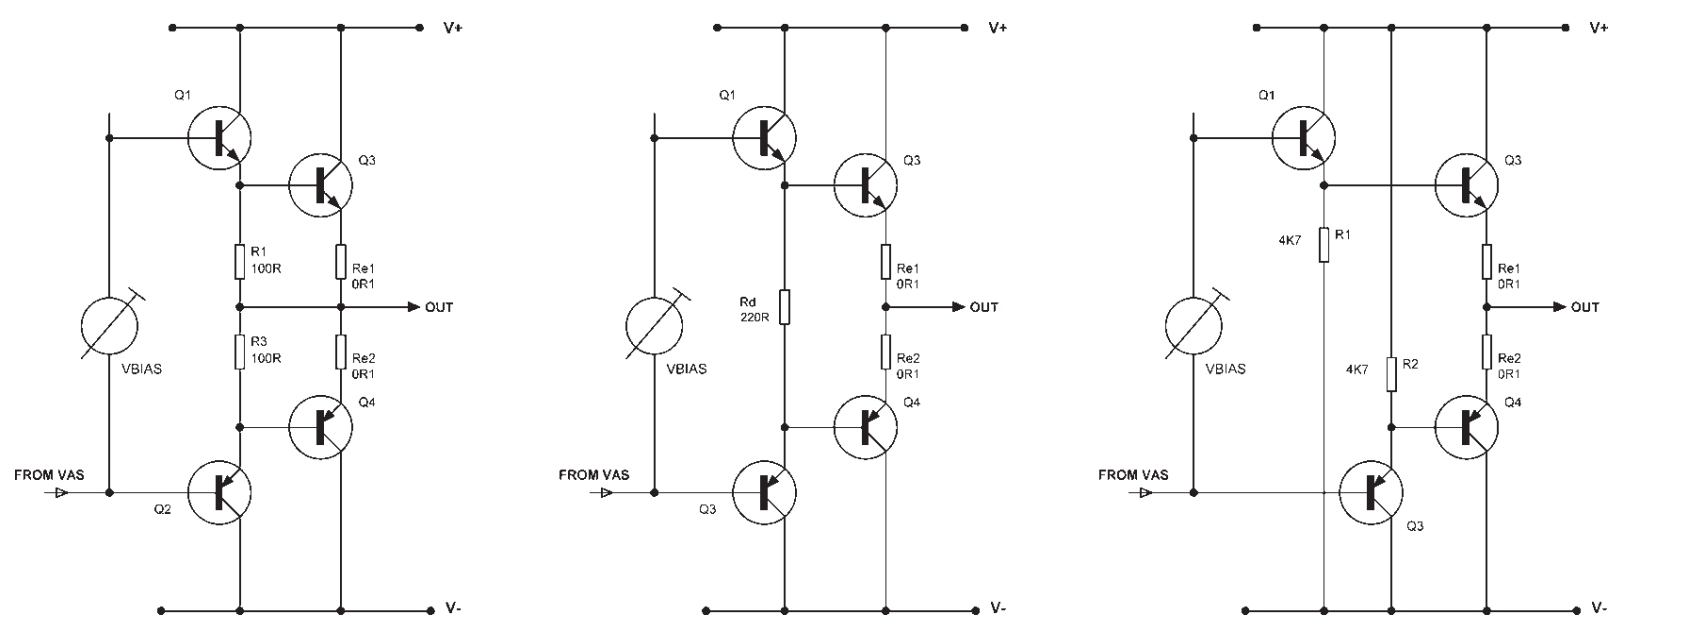
\includegraphics[width=\textwidth]{ImagenesOutput-Stage/pag143-EF.png}
	\caption{Tipos de configuraciones emitter follower. D. Self, Audio Power Amplifier Design Handbook, 5th, p. 143.}
	\label{fig:ef}
\end{figure}


Otra configuración involucra los pares Sziklai, Quasi-Darlington o también llamados par de realimentación, dado que ahora el driver se coloca de manera tal que este compare la tensión a la salida con la entrada, lo cual aumenta la linealidad. Además, como el Vbe del transistor de salida se encuentra dentro del lazo de realimentación, se observa una estabilidad térmica mayor.

%, trim = {0 0 0 20},clip
\begin{figure}[H]
\centering
	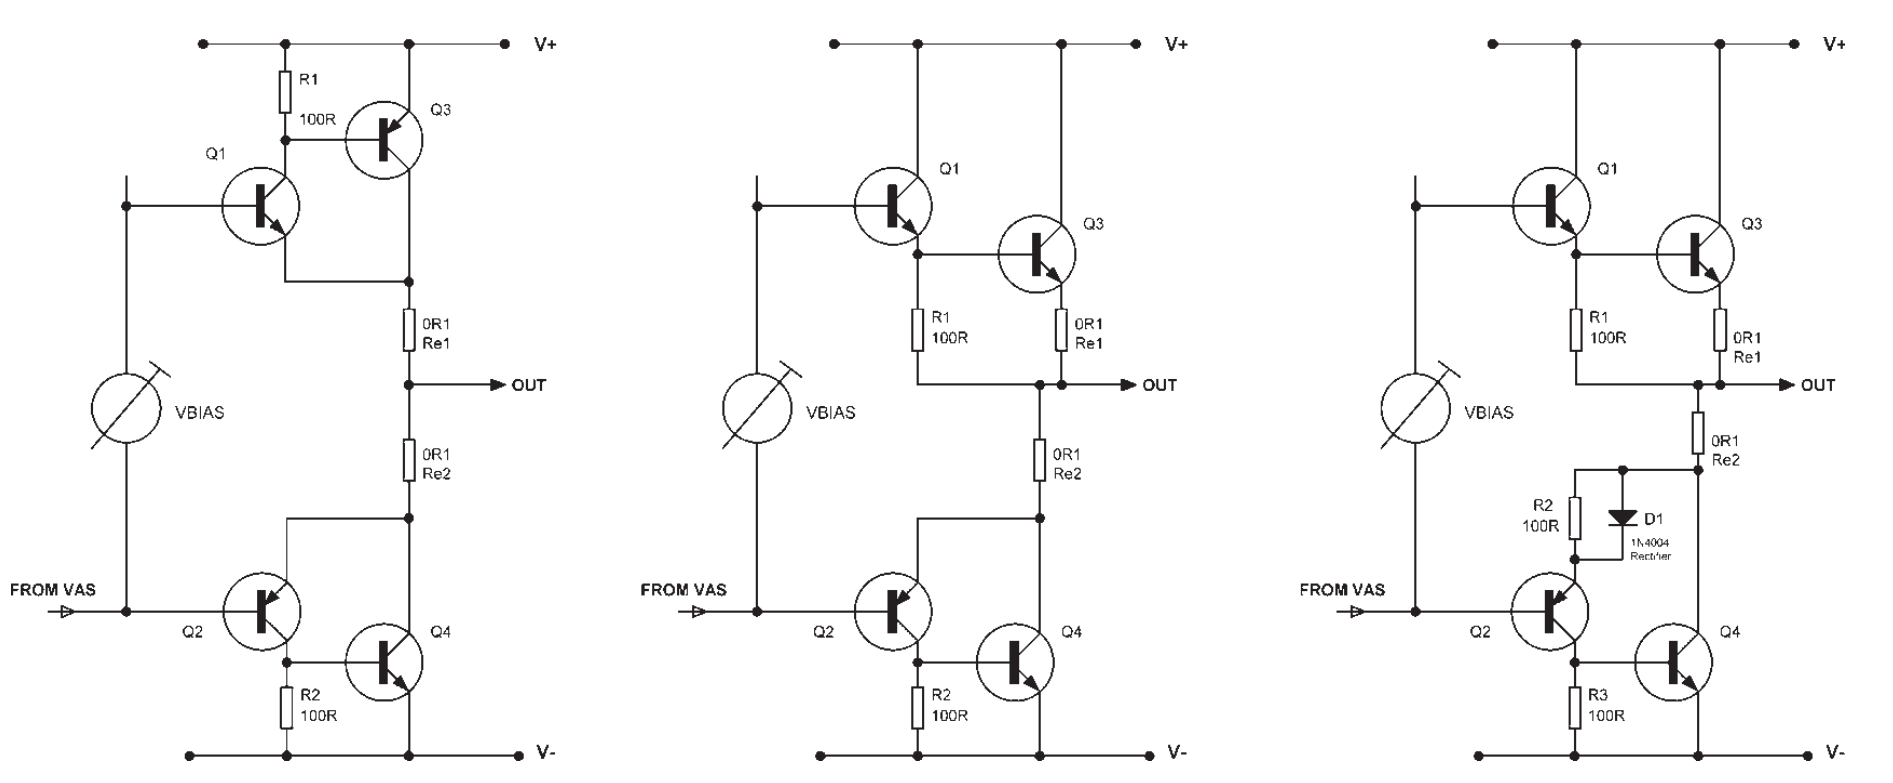
\includegraphics[width=\textwidth]{ImagenesOutput-Stage/pag145-CFP.png}
	\caption{Tipos de configuraciones de par de realimentación. D. Self, Audio Power Amplifier Design Handbook, 5th, p. 145.}
	\label{fig:cfp}
\end{figure}

Una topología la cual en el pasado era casi obligatoria por la falta de transistores PNP de potencia complementarios a los NPN, es la casi complementaria. En esta configuración solamente se reemplaza por un par Quasi-Darlington a los transistores PNP. Esta topología presenta una linealidad mucho menor y no será utilizada, aunque existen varios arreglos a la simetría, como por ejemplo utilizando un diodo de Baxandall.

Naturalmente surge al analizar estas etapas de salida la idea de colocar tres transistores en cascada, o más. De ahí surge la topología basada en triples, como la Triple EF. Esta configuración presenta mayor linealidad a alta potencias, un punto Q más estable para los transistores \textit{pre-drivers}, los que proporcionan la corriente a los drivers, debido a que estos manejarán una corriente menor y disiparán menor potencia. Además, al poseer una ganancia de corriente mayor, la etapa de ganancia de tensión deberá proporcionar corrientes menores. En la Figura (\ref{fig:triples}) se observan distintas configuraciones triples posibles.

%, trim = {0 0 0 20},clip
\begin{figure}[H]
\centering
	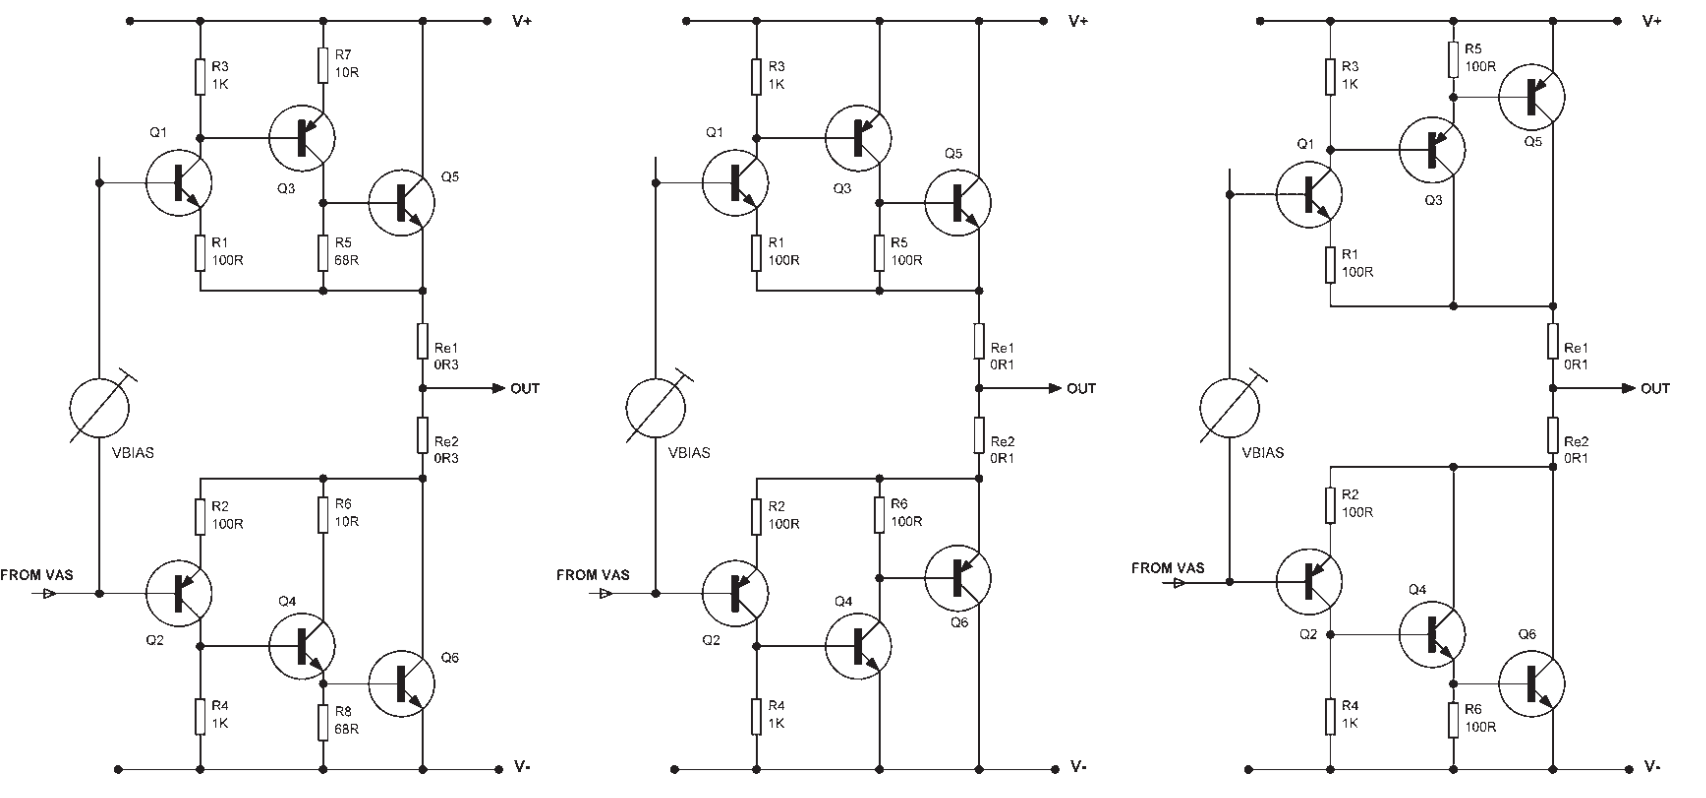
\includegraphics[width=\textwidth]{ImagenesOutput-Stage/pag145-triples.png}
	\caption{Algunos tipos de configuraciones basadas en triples. D. Self, Audio Power Amplifier Design Handbook, 5th, p. 145.}
	\label{fig:triples}
\end{figure}

\subsubsection{Topología Utilizada}
Debido a la alta potencia que se deberá disipar sobre la carga, que al ser de tan solo $8 \ \Omega$ provoca corrientes muy grandes, se decidió utilizar una topología basadas en triples detallado en la Figura (\ref{fig:triples}). Esto permite, como ya descrito antes, utilizar transistores de baja potencia como pre-drivers que tanto permanezcan a una temperatura estable como posean una pequeña excursión en corriente, lo que aumenta la linealidad de la etapa de salida. Luego, el transistor driver y de salida serán de potencia. Se utilizará una configuración con pares de realimentación para aumentar aún más la linealidad.

 %, trim = {0 0 0 20},clip
\begin{figure}[H]
\centering
	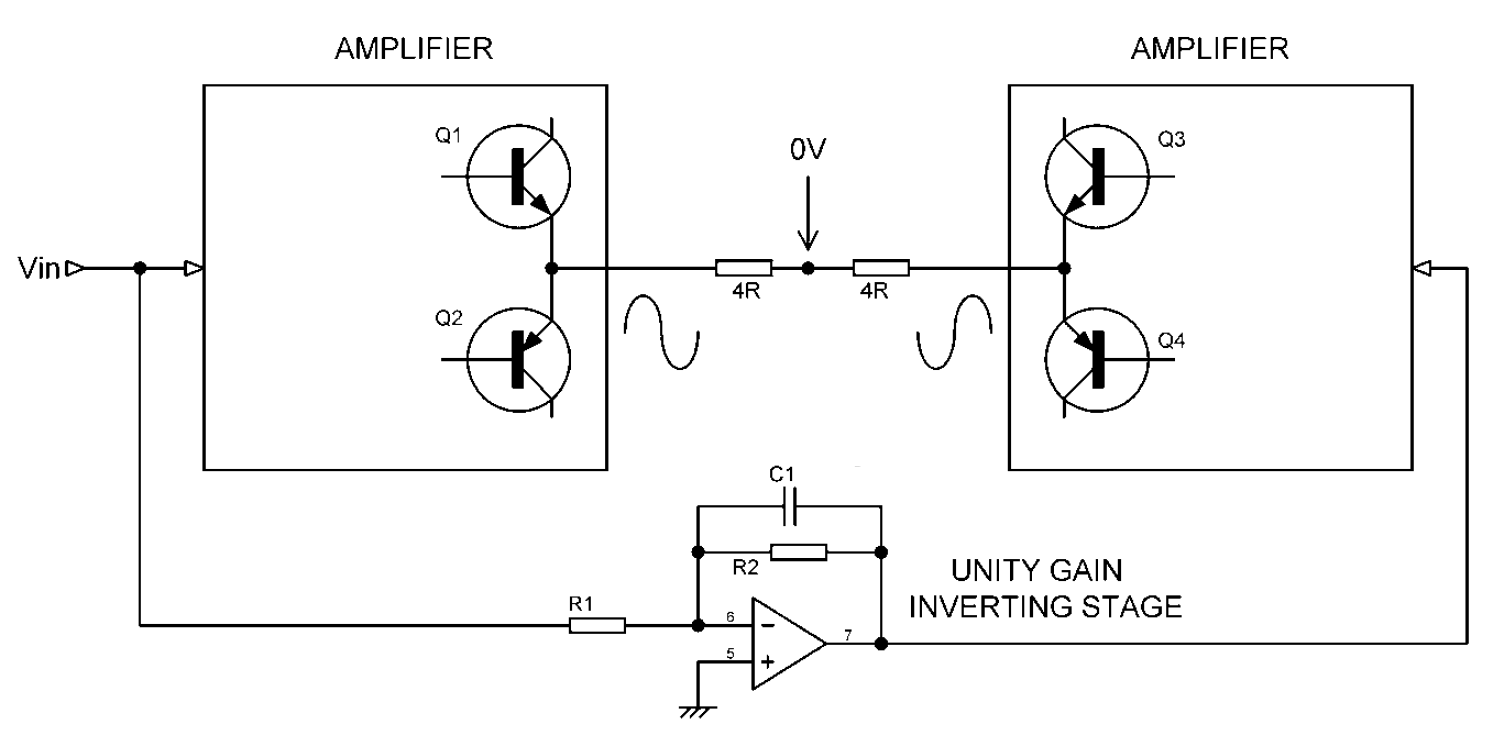
\includegraphics[width=0.7\textwidth]{ImagenesOutput-Stage/pag38-bridge.png}
	\caption{Puenteo de la carga con las etapas de salida. D. Self, Audio Power Amplifier Design Handbook, 5th, p. 38.}
	\label{fig:bridge}
\end{figure}

Por otro lado, debido a que el amplificador diseñado será para una carga mono y no estéreo, se utilizaron dos etapas de salida idénticas pero en contra-fase con la carga entre la salida de ambas. Esto permite duplicar la tensión sobre la carga y así cuadriplicar la potencia disipada sobre esta.
Como la potencia disipada será muy alta, se decidió utilizar además una técnica muy frecuentemente usada en amplificadores de audio comerciales, la cual consiste en colocar varios transistores de salida en paralelo, pudiendo haber incluso quince de ellos. El número de transistores en paralelo se decidirá en la sección de potencia.



\subsubsection{Generador de Bias}

Para el generador de bias se utilizó inicialmente un multiplicador de Vbe compuesto por dos resistencias y un transistor. Sin embargo, resultados experimentales demostraron que este generador de bias fallaba en mantener una tensión constante de bias frente a las grandes variaciones de corriente que egresaban de la etapa de salida. Debido a esto, se utilizó un par de realimentación compensado en vez del transistor, lo cual aumenta el beta total, logrando generar una tensión de bias con una fluctuación alrededor de diez veces menor.

 %, trim = {0 0 0 20},clip
\begin{figure}[H]
\centering
	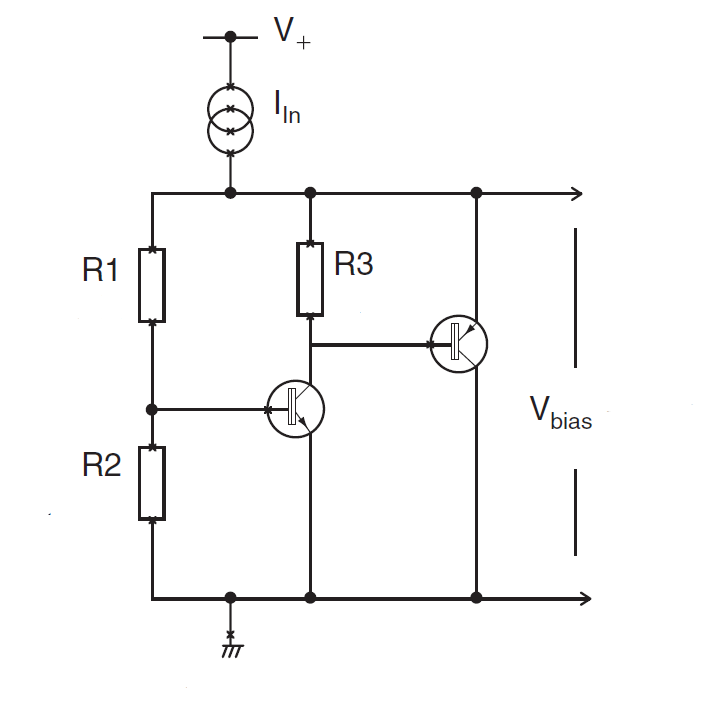
\includegraphics[width=0.4\textwidth]{ImagenesOutput-Stage/pag417-bias.png}
	\caption{Generador de bias utilizado. D. Self, Audio Power Amplifier Design Handbook, 5th, p. 417.}
	\label{fig:bias}
\end{figure}

La corriente que fluye por las resistencias $R_1$ y $R_2$ está gobernada por tanto la caída de $V_{be}$ como por el valor de $R_2$. Imponiendo una corriente de $2 \ mA$ para estas resistencias, se tiene que

\begin{equation}
I_R = \frac{0.6 \ V}{2 \ mA} = 300 \ \Omega
\end{equation}

Luego, dado que se encuentran seis caídas de $V_{be}$, lo cual equivale a $4.2 \ V$, se decidió para poder ajustar el nivel de corriente de reposo de los transistores de salida, tomar ese valor como central y con un trimmer brindar una excursión bilateral frente este valor central. Si el trimmer se coloca en la posición de menor resistencia, habrá una gran distorsión de crossover, mientras que si se coloca en la posición de mayor resistencia habrá una gran corriente de reposo. Teniendo esto en cuenta, se tiene que $R_2 = R_{2-fija} + R_{2-trimmer}$. $R_{2-fija} = 1.5 \ k\Omega$ y $R_{2-trimmer} = 500 \ \Omega$ nominales. Esto hará que

\begin{equation}
3.6 \ V < V_{bias} < 4.6 \ V
\end{equation} 

\subsubsection{Fuente de corriente}

Finalmente, se utilizó una fuente de corriente compensada simple en vez de una resistencia para no limitar por corriente a la máxima potencia sin recorte a la salida. Esta fuente de corriente será la que provea de corriente a tanto el generador de Bias como a los transistores pre-driver de salida. Para el valor de la fuente de corriente se decidió utilizar $7 \ mA$ dado que eso brinda suficiente margen entre la corriente de base del transistor pre-driver ($\approx 1 \ mA$) y el generador de bias. Se cedieron alrededor de $6 \ mA$ al generador de bias para no solo dejar una buena corriente de colector en los transistores, sino también dejar una corriente sobre las resistencias para que valga la aproximación de divisor resistivo. Se obtuvo entonces que la resistencia que fija la corriente de la compensada es
\begin{equation}
R_{curr} = \frac{0.7 \ V}{7 \ mA} = 100 \ \Omega
\end{equation}
Finalmente para polarizar correctamente los diodos, como se colocaron cuatro transistores en paralelo a estos, se impuso una corriente mayor a la habitual, de $20 \ mA$. Obteniendo así
\begin{equation}
R_{diod} = \frac{0.7 \ V}{20 \ mA} = 3k3 \ \Omega
\end{equation}

\subsubsection{Resistor sumidero de corriente}

Por esta resistencia fluirá la resta de corrientes entre la proporcionada por la fuente de corriente compensada descrita anteriormente y la fuente de corriente JFET, la cual cumple la función de acople entre el VAS y la etapa de salida, y de ajuste de continua en la carga. Se tiene luego que $7 \ mA - 5 \ mA = 2 \ mA$. Luego,

\begin{equation}
R = \frac{V_{output_{max}}}{I_R} = \frac{45 \ V}{2 \ mA} = 22.5 \ k\Omega 
\end{equation} 

Sin embargo, se comprobó empíricamente mediante simulaciones que un valor de $R = 25 \ k\Omega$ decrece la distorsión armónica sin comprometer mucho el funcionamiento.

\end{document}